\section{Soběpodobnost}\label{sec:sobepodobnost}
Mandelbrot si uvědomil, že struktura pobřeží se charakterově vymyká útvarům do tehdy známým eukleidovské geometrii, neboť mapy s různými měřítky poskytovaly různou úroveň detailů, které hrály netriviální roli v jeho celkové délce. Učinil však jiné zásadní pozorování, a to sice, že mnoho detailů má společné rysy, které se opakují. Hodně z nich se shodovalo s výjimkou jejich měřítka. \citep[str. 96]{Mandelbrot1983}\par

Ve fraktální geometrii se pro tento úkaz uchytil termín \emph{soběpodobnost} (angl. \emph{self-similarity}). Útvar nazýváme soběpodobným, \textbf{pokud se sám sobě podobný v libovolném měřítku} \citep[str. 220]{Voracova2022} nebo pokud \textbf{část útvaru je podobná jeho celku}. Zmíněná podoba může být míněna přibližně (např. v případě pobřeží je nejspíše jasné, že žádné z jeho detailů nesdílejí společné rysy přesně), ale v dalších částech si předvedeme soběpodobnost \emph{přímou}.

\subsection{Kochova křivka}\label{subsec:kochova_krivka}
Jak jsme si již uvedli, za otce fraktální geometrie je považován Mandelbrot, avšak mnoho fraktálních křivek bylo známo již dříve (čtenář promine, že jsme zatím blíže nespecifikovali termín ``fraktální'', jeho význam pro nás však zatím nebude stěžejní). Jako první se podíváme na jednu z nejznámějších, kterou objevil roku \emph{1904} švédský matematik \name{Helge~von~Koch} \mbox{(1870--1924)}, dnes známou pod názvem \emph{Kochova křivka}. \citep[str. 61]{Peitgen2004} Na začátku vezmeme úsečku délky $1$. Vyjmeme prostřední (tj. druhou) třetinu a nahradíme ji dvěma úsečkami délky $1/3$, tak, aby na sebe navazovaly v krajních bodech. Tento proces následně opakujeme pro nově vzniklé úsečky. Obecně u úsečky délky $l$ nahradíme její prostřední třetinu dvojicí úseček délek $l/3$ (viz obrázek \ref{fig:kochova_vlocka_5iteraci}).
\begin{figure}[h]
    \centering
    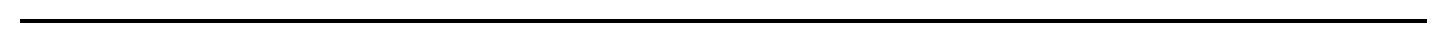
\includegraphics[scale=\fractalscale]{ch01_kochova_krivka_0iterace.pdf}\\\qquad\\
    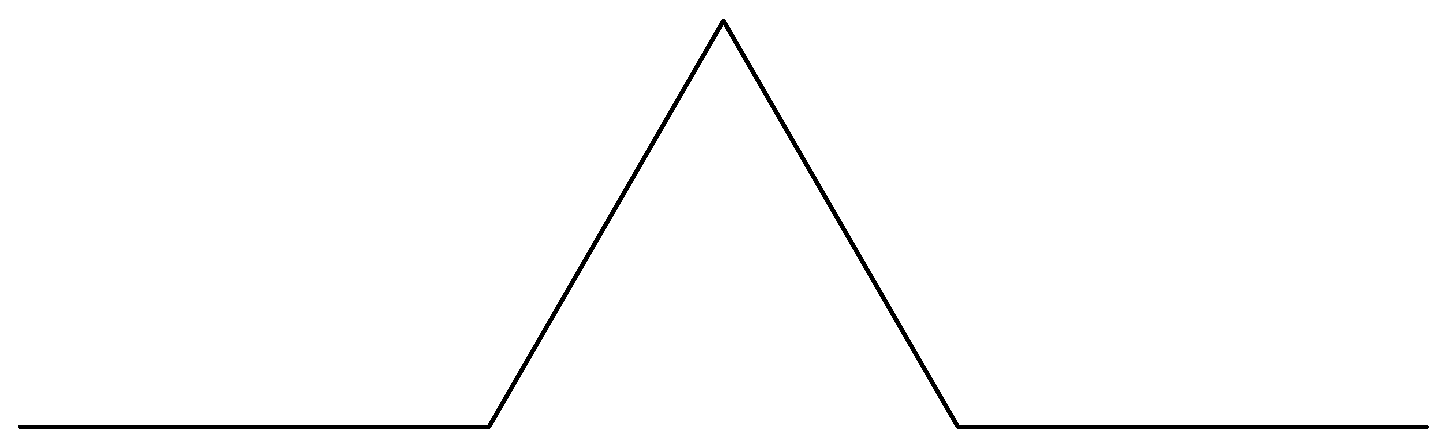
\includegraphics[scale=\fractalscale]{ch01_kochova_krivka_1iterace.pdf}\\\qquad\\
    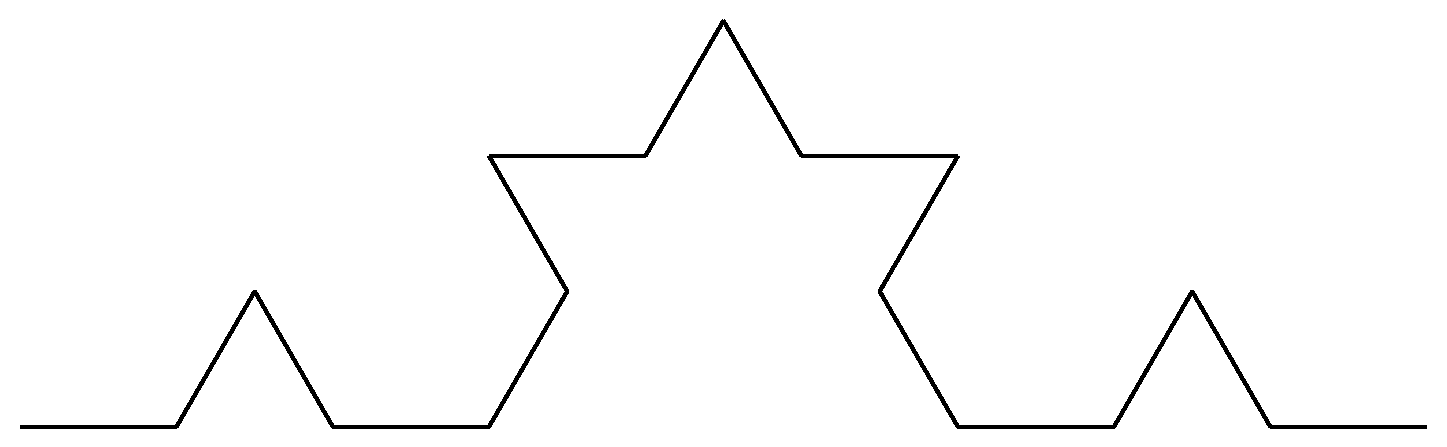
\includegraphics[scale=\fractalscale]{ch01_kochova_krivka_2iterace.pdf}\\\qquad\\
    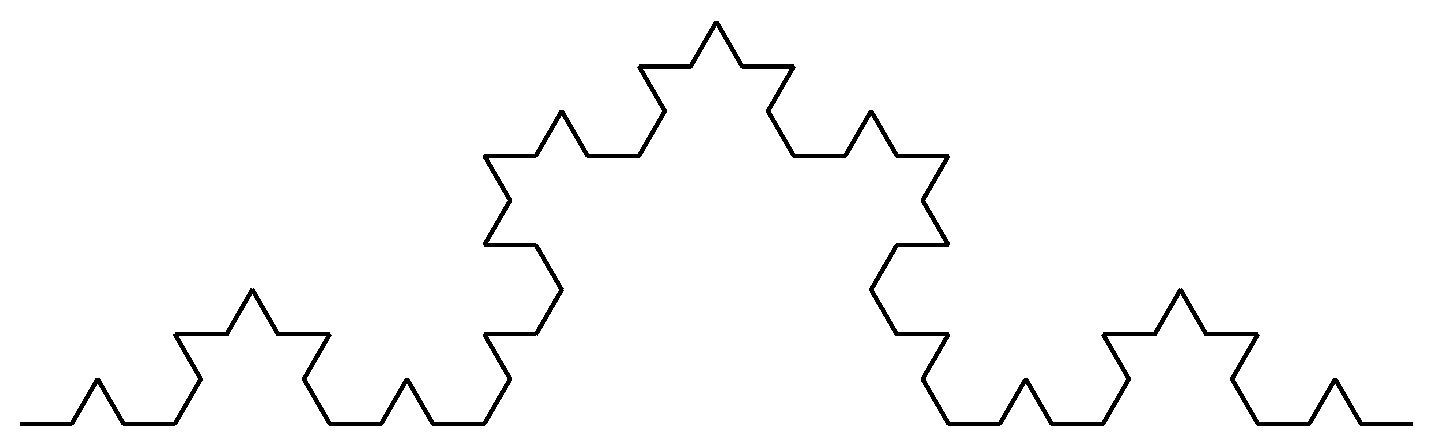
\includegraphics[scale=\fractalscale]{ch01_kochova_krivka_3iterace.pdf}\\\qquad\\
    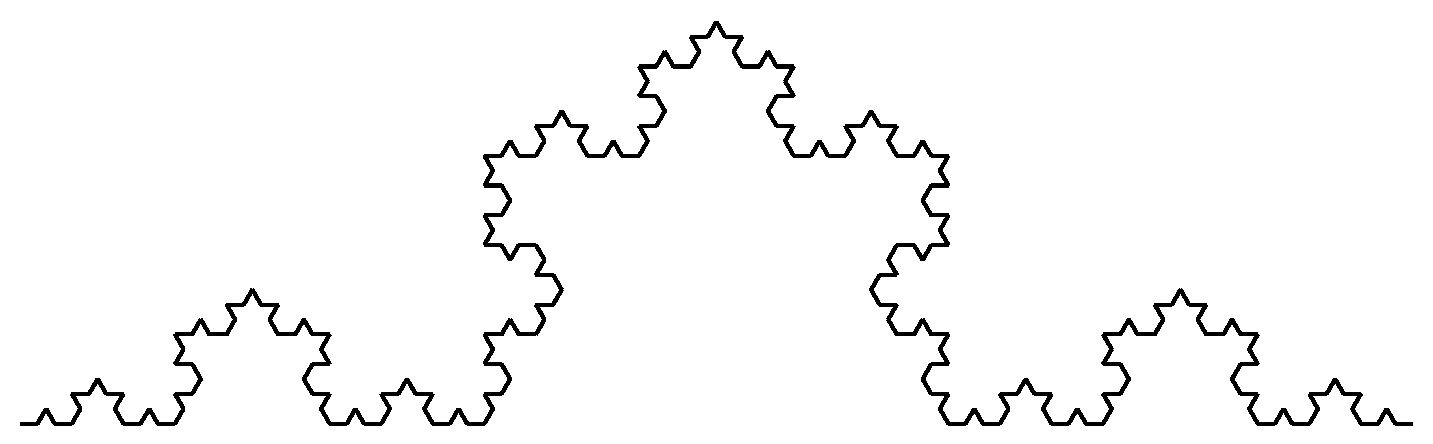
\includegraphics[scale=\fractalscale]{ch01_kochova_krivka_4iterace.pdf}\\\qquad\\
    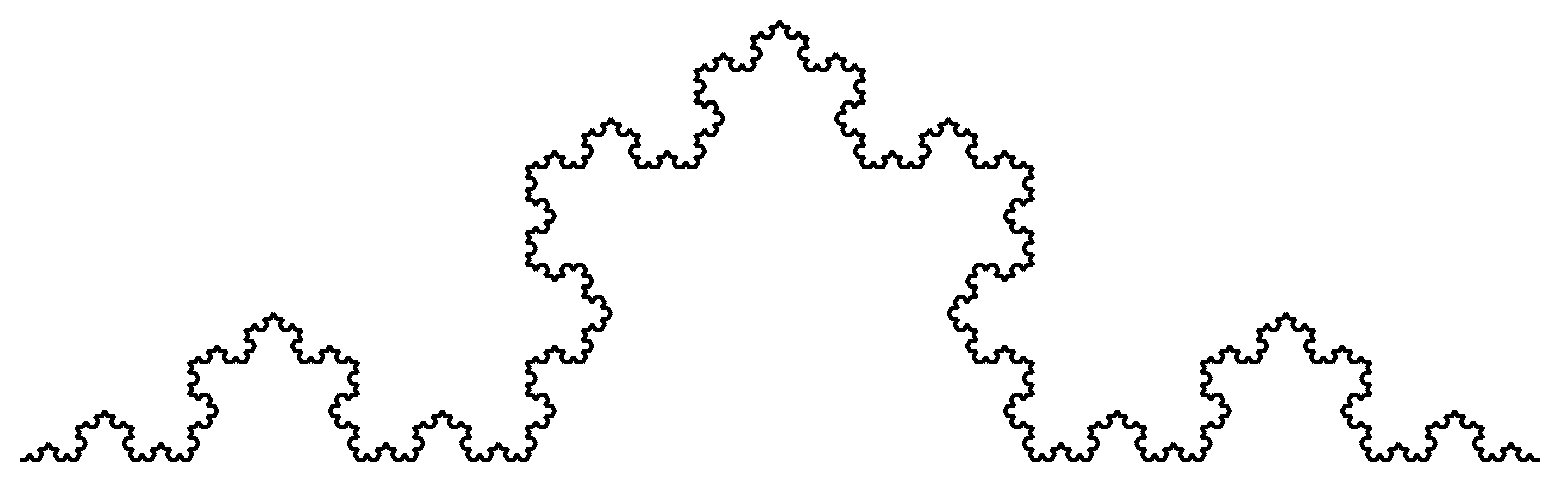
\includegraphics[scale=\fractalscale]{ch01_kochova_krivka_5iterace.pdf}
    \caption{Prvních pět iterací Kochovy křivky.}
    \label{fig:kochova_vlocka_5iteraci}
\end{figure}
V první řadě si můžeme všimnout, že v každé další iteraci jsou nově vzniklé podobné původnímu celku, tedy v předešlé iteraci (viz obrázek \ref{fig:kochova_krivka_podobnost}). Pokud by tento proces pokračoval do nekonečna, pak by každá ze čtyř částí křivky představovala \textbf{celý původní obrazec} ve zmenšeném měřítku (byla by tedy soběpodobná).
\begin{figure}[h]
    \centering
    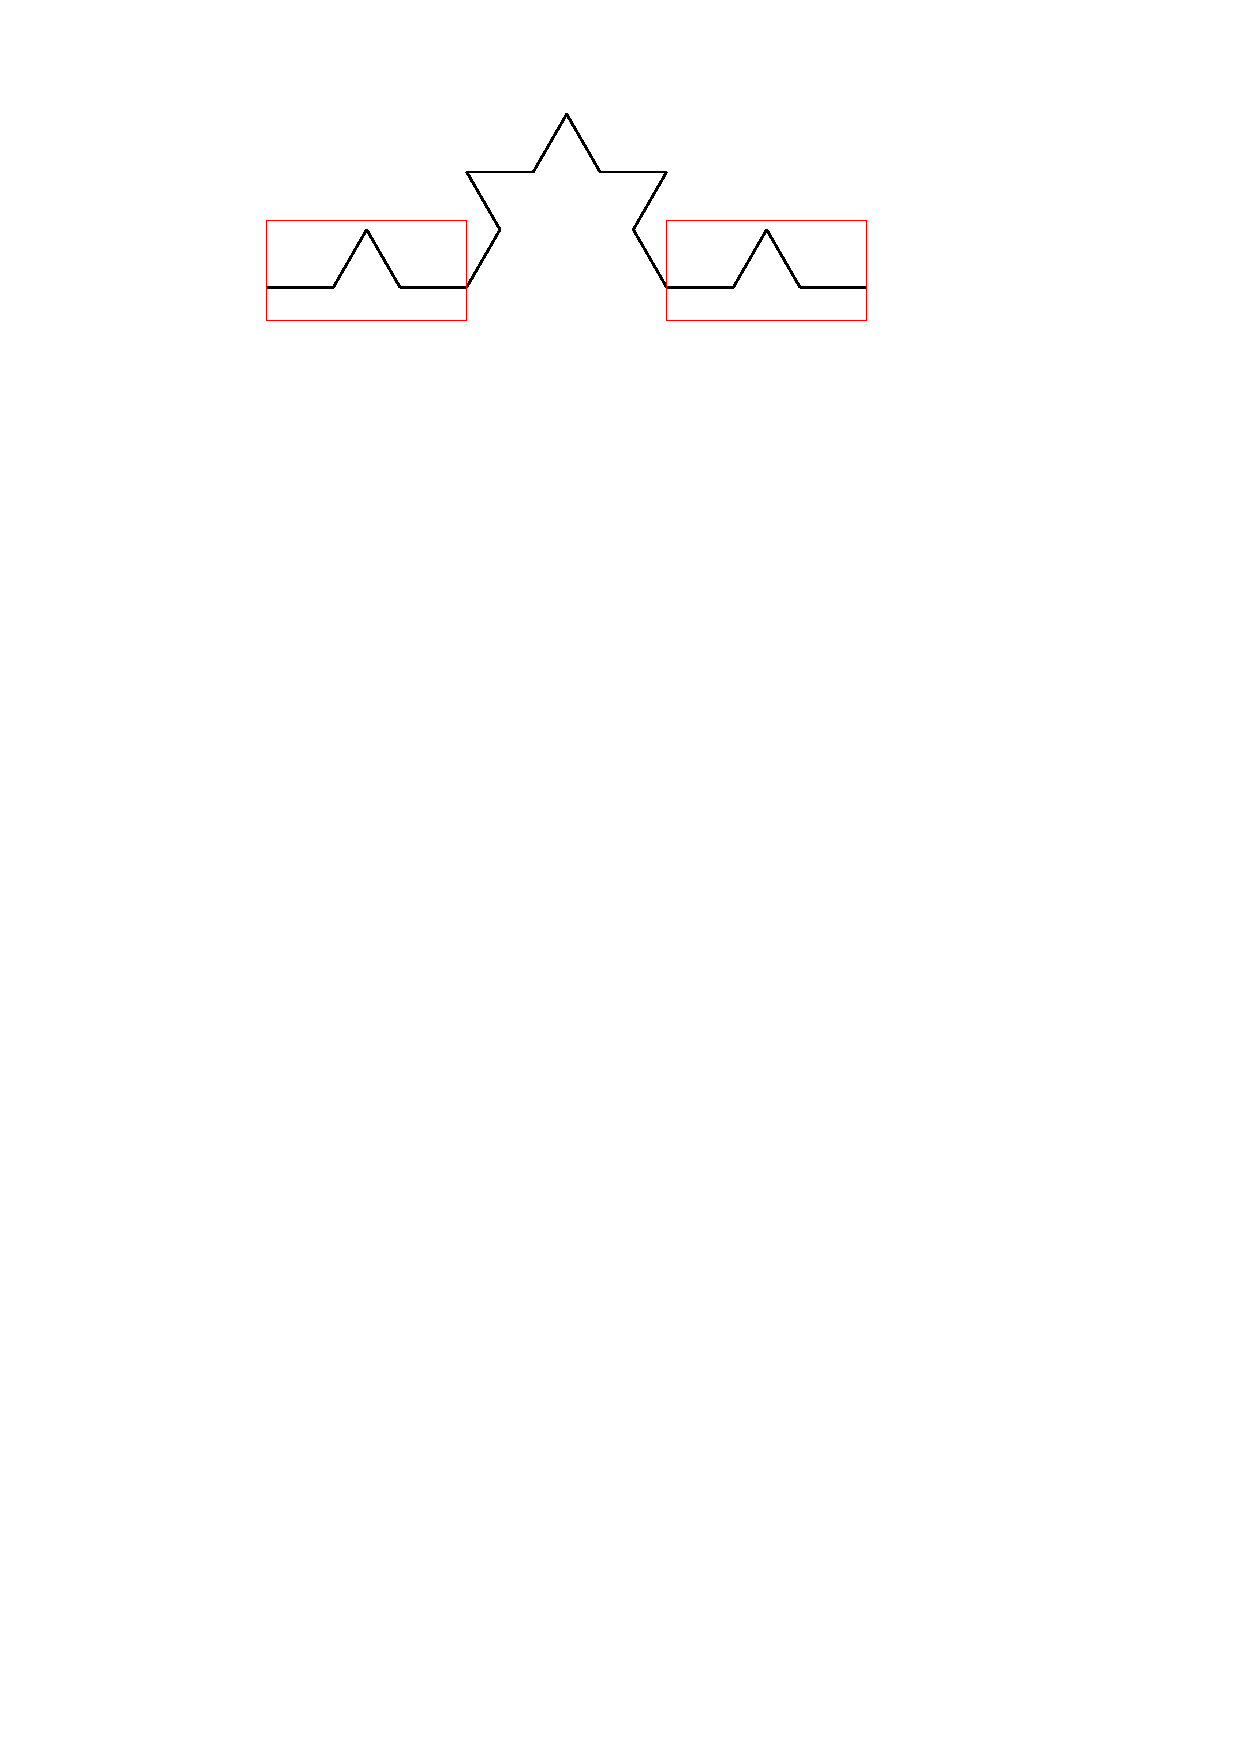
\includegraphics[scale=\normalipe]{ch01_kochova_krivka_podobnost.pdf}
    \caption{První iterace Kochovy křivky ``uvnitř'' druhé v menším měřítku.}
    \label{fig:kochova_krivka_podobnost}
\end{figure}
Zkusme se nyní podívat na délku křivky. V první iteraci začínáme s úsečkou délky\footnote{Mohli bychom také začít s obecnou délkou $\ell_0$, ale ta by se však při výpočtu projevila pouze jako konstantní násobek.} $1$, která se v druhé iteraci změní na křivku délky $4/3$. Není těžké si rozmyslet, že obecně v $n$-té iteraci bude délka křivky $\ell_n$ rovna
\begin{equation*}
    \left(\dfrac{4}{3}\right)^{n}.
\end{equation*}
Posloupnost $\{\ell_n\}_{n=1}^{\infty}$ je geometrická s kvocientem $4/3>1$, a tedy její limita je $\infty$. Kochova křivka má tak nekonečnou délku.

\subsection{Sierpińského trojúhelník}\label{subsec:sierpinskeho_trojuhelnik}


\subsection{Kochova vločka}\label{subsec:kochova_vlocka}
Rozšiřující variantou Kochovy křivky \ref{subsec:kochova_krivka} je tzv. \emph{Kochova vločka}, která se skládá ze tří Kochových křivek. Rozdíl je zde v tom, že začínáme s rovnostranným trojúhelníkem o straně délky $1$. Na každou ze stran aplikujeme stejný proces, jako předtím, tj. odebereme prostřední třetinu, nahradíme ji dvěma na sebe navazujícími úsečkami délek $1/3$ a opakujeme pro každou nově vzniklou úsečku (viz obrázky \ref{fig:kochova_vlocka_dve_iterace} a \ref{fig:kochova_krivka_5iterace}).
\begin{figure}[h]
    \centering
    \begin{subfigure}{\subfigwidth}
        \centering
        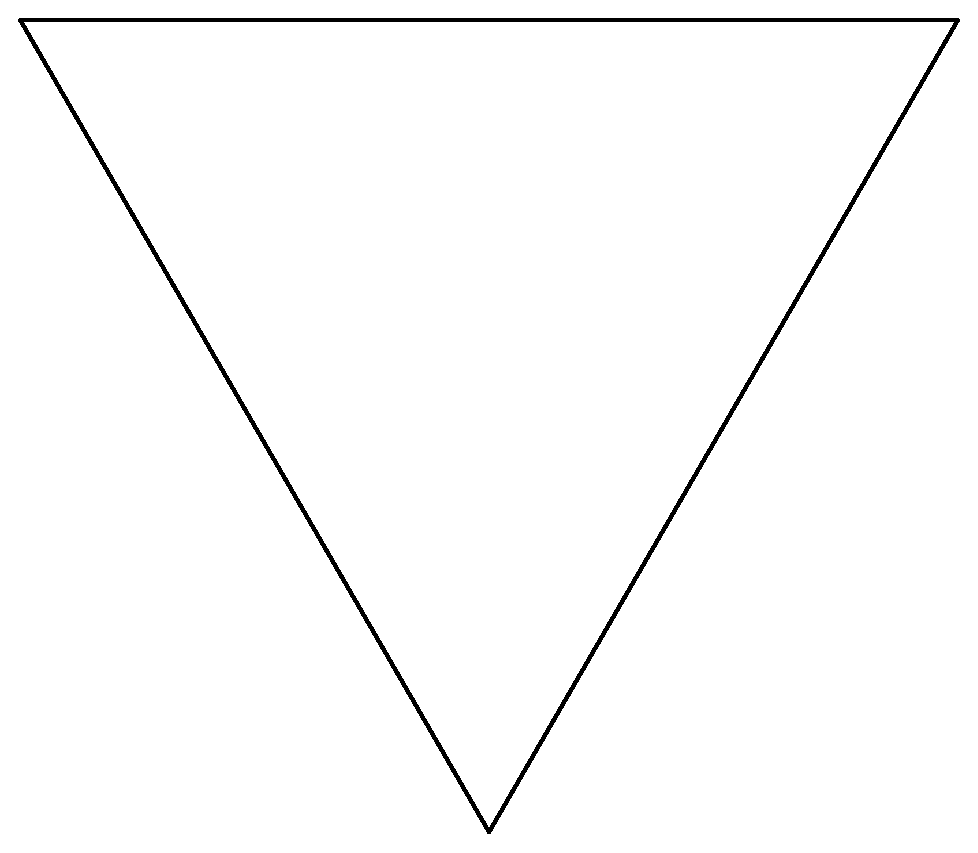
\includegraphics[scale=\fractalscale]{ch01_kochova_vlocka_0iterace.pdf}
    \end{subfigure}
    \qquad
    \begin{subfigure}{\subfigwidth}
        \centering
        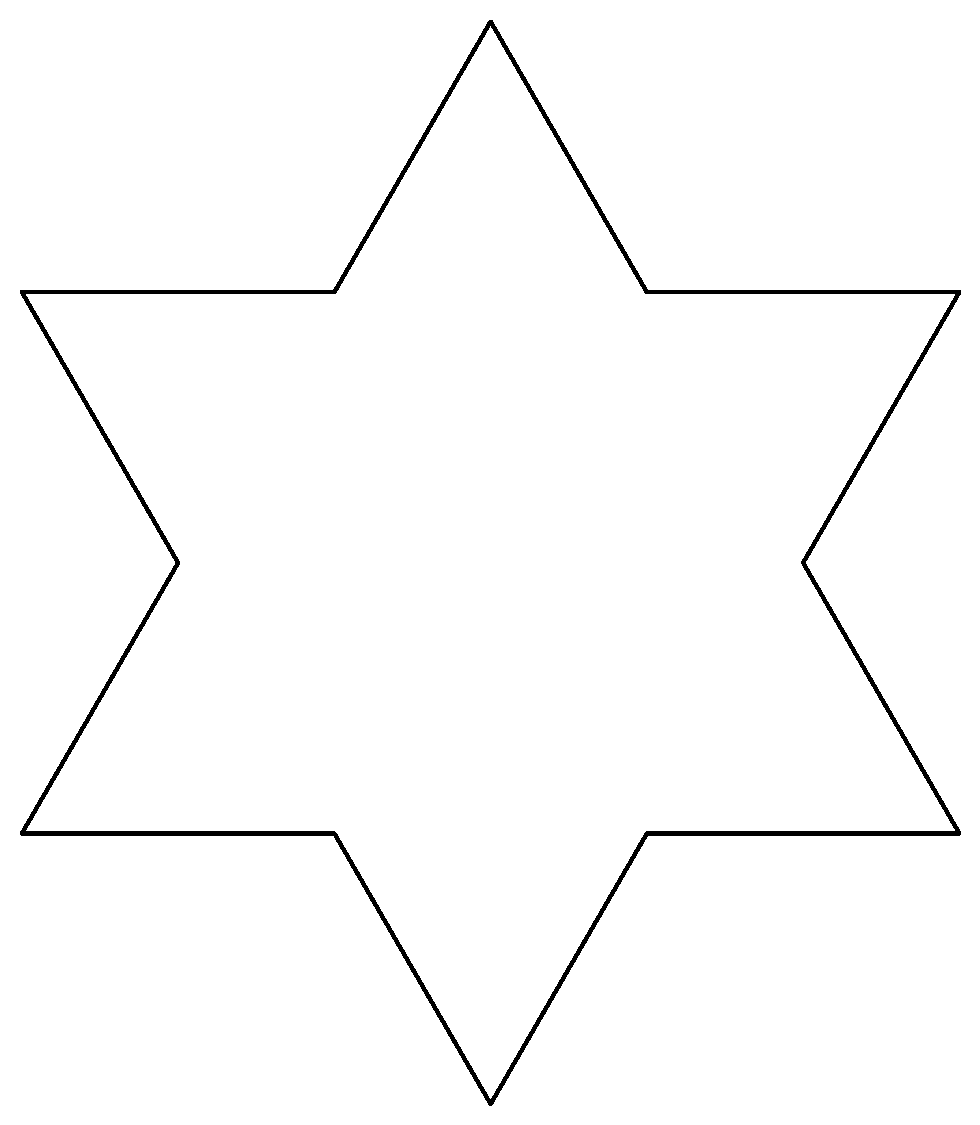
\includegraphics[scale=\fractalscale]{ch01_kochova_vlocka_1iterace.pdf}
    \end{subfigure}
    \caption{Nultá a první iterace Kochovy vločky.}
    \label{fig:kochova_vlocka_dve_iterace}
\end{figure}
\begin{figure}[h]
    \centering
    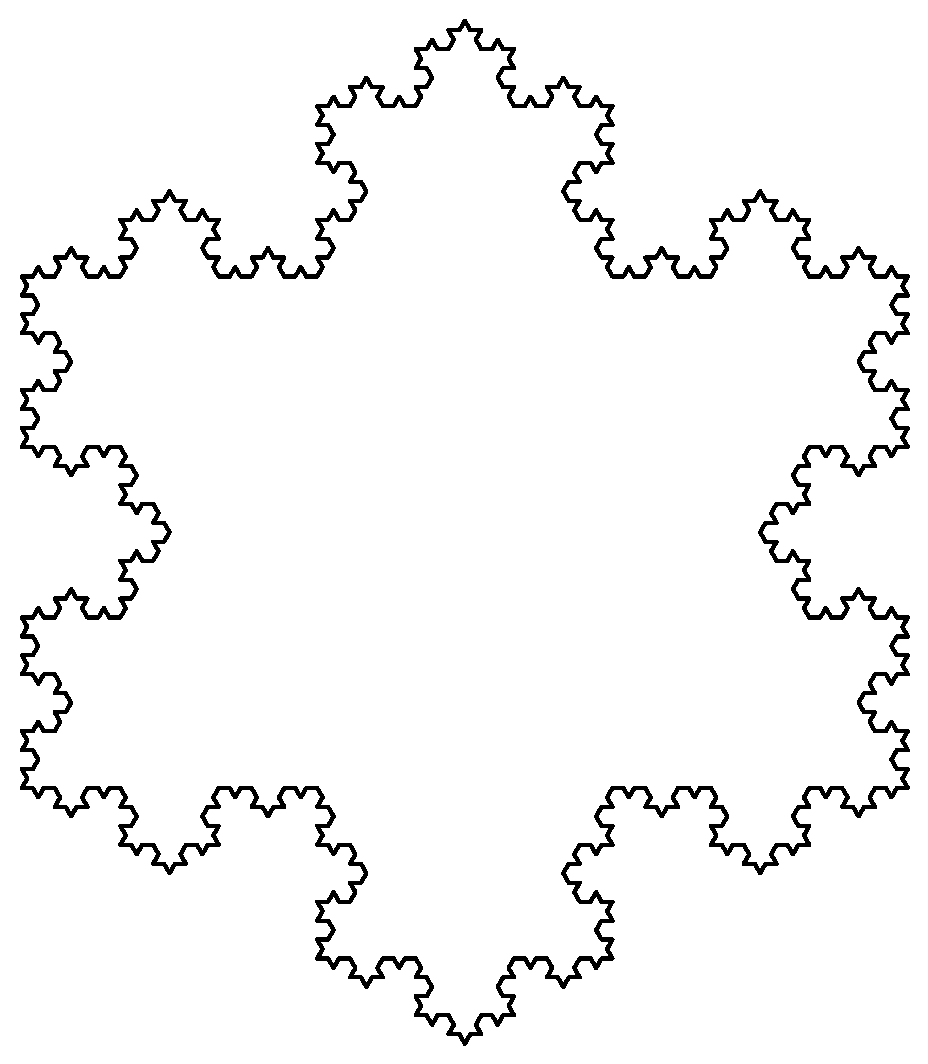
\includegraphics[scale=\fractalscale]{ch01_kochova_vlocka_4iterace.pdf}
    \caption{Čtvrtá iterace Kochovy vločky.}
    \label{fig:kochova_krivka_5iterace}
\end{figure}
Podíváme-li se na obvod, nejspíše nás již nepřekvapí, že i zde je nekonečný\footnote{Obvod Kochovy křivky po $n$-té iteraci je $o_n=3\cdot(4/3)^{n}$.} (už z principu, že každá strana původního rovnostranného trojúhelníka představuje samostatnou Kochovu křivku). Obsah vzniklého útvaru je však již zajímavější. Lze snadno odvodit, že obsah rovnostranného trojúhelníku o straně délky $a$ je
\begin{equation*}
    \dfrac{\sqrt{3}}{4}a^2
\end{equation*}
Na začátku je obsah útvaru $S_0=\sqrt{3}/4$. Po první iteraci přibudou 3 nové trojúhelníky se stranou délky $1/3$, tzn. jejich obsah bude
\begin{equation*}
    \dfrac{\sqrt{3}}{4}\left(\dfrac{1}{3}\right)^2
\end{equation*}
a celkový obsah obrazce tedy bude
\begin{equation*}
    S_1=\dfrac{\sqrt{3}}{4}+3\cdot\dfrac{\sqrt{3}}{4}\left(\dfrac{1}{3}\right)^2.
\end{equation*}
V každé další iteraci vzniknou z jedné úsečky 4 nové. Obecně po $n$ iteracích jich bude $3\cdot 4^n$ (při výpočtu však musíme počítat s o jedna nižší mocninou, neboť trojúhelníky vznikají ``na úsečkách'' z předešlé iterace, nikoliv té aktuální, viz obrázek \ref{fig:kochova_vlocka_2iterace_nove_trojuhelniky}).
\begin{figure}[h]
    \centering
    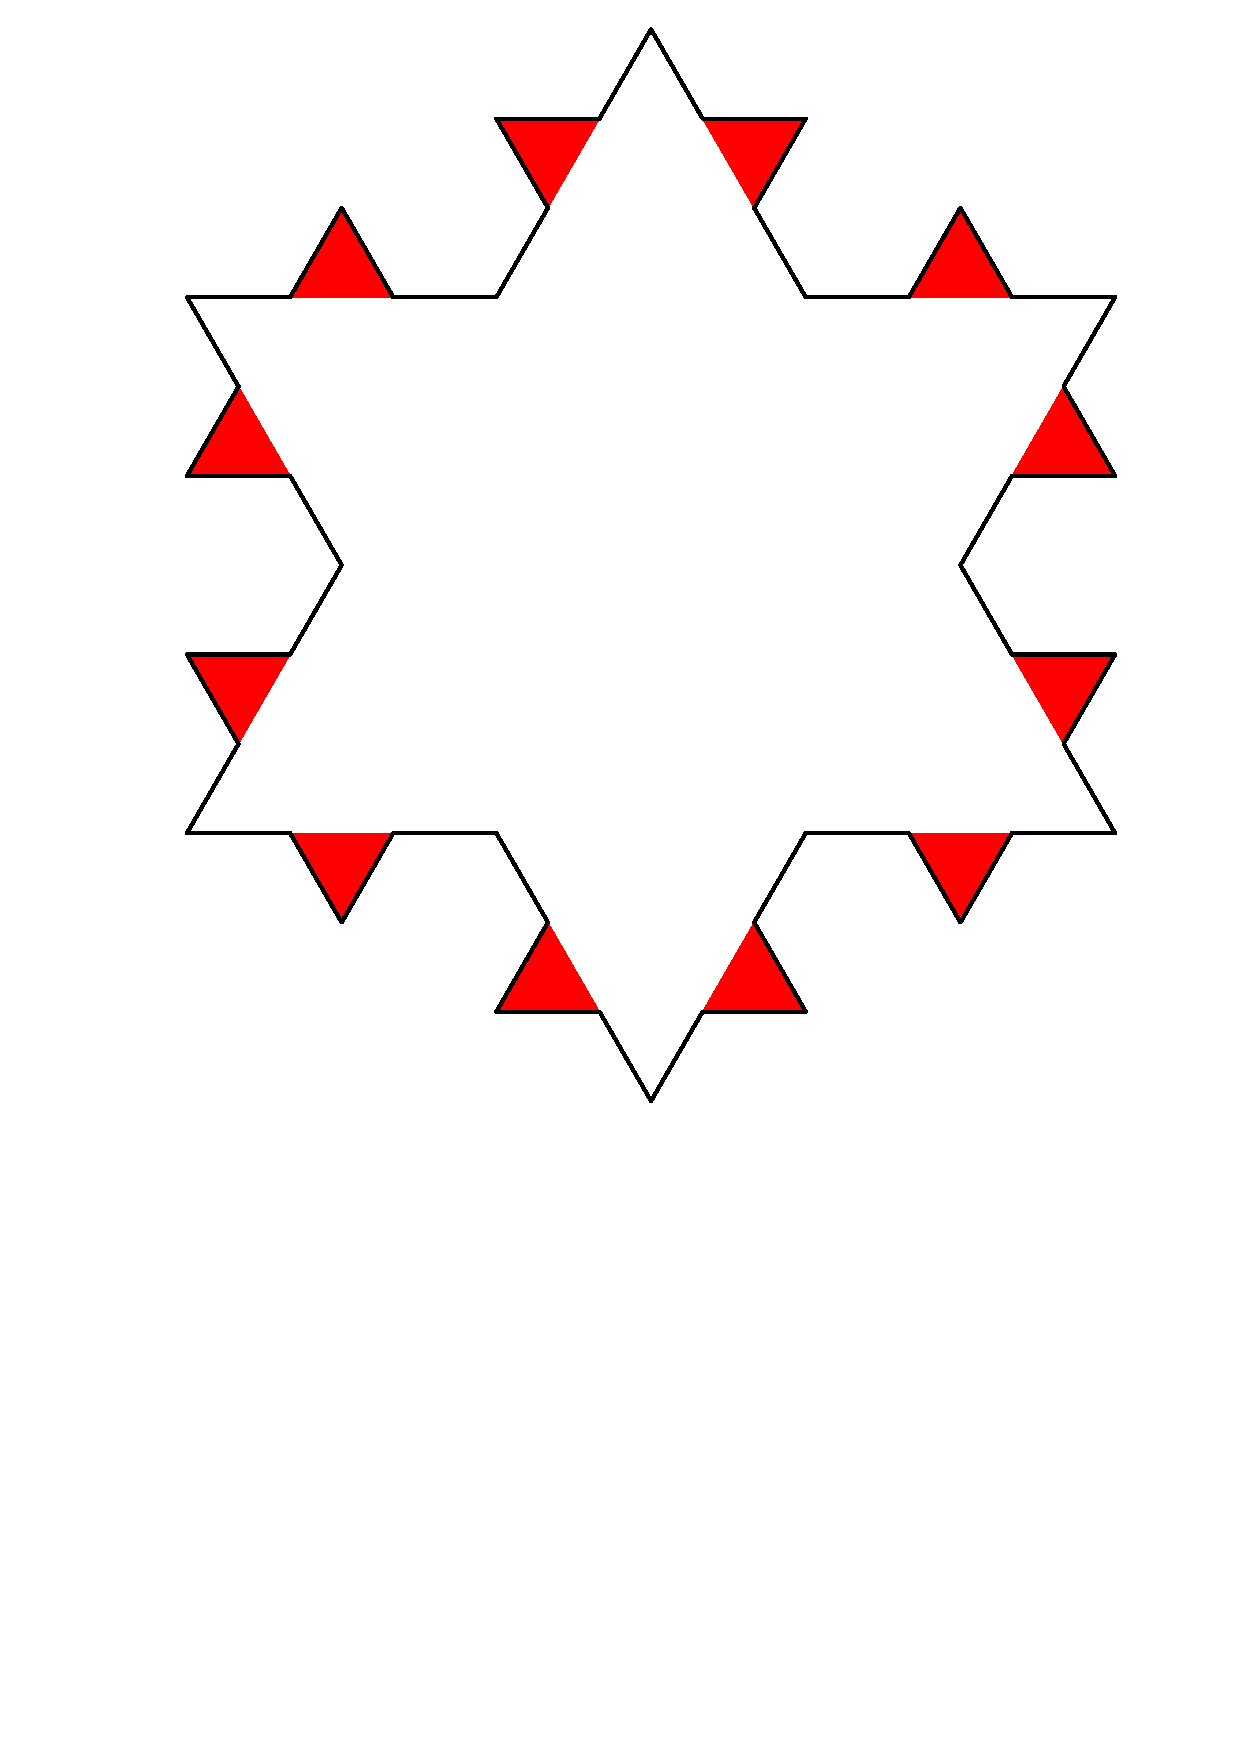
\includegraphics[scale=\fractalscale]{ch01_kochova_vlocka_2iterace_nove_trojuhelniky.pdf}
    \caption{Nově vzniklé trojúhelníky v druhé iteraci.}
    \label{fig:kochova_vlocka_2iterace_nove_trojuhelniky}
\end{figure}
Délka úseček, a tedy i stran nově vzniklých rovnostranných trojúhelníků, je $(1/3)^n$. Celkový obsah nově vzniklých trojúhelníků je tak
\begin{equation}\label{eq:obsah_novych_trojuhelniku}
    3\cdot 4^{n-1}\cdot\dfrac{\sqrt{3}}{4}\left(\dfrac{1}{3^n}\right)^2.
\end{equation}
Pro další výpočet bude pro nás výhodné si výraz \eqref{eq:obsah_novych_trojuhelniku} upravit.
\begin{equation*}
    3\cdot 4^{n-1}\cdot\dfrac{\sqrt{3}}{4}\left(\dfrac{1}{3^n}\right)^2=\dfrac{3\sqrt{3}}{4^2}\cdot \dfrac{4^n}{3^{2n}}=\dfrac{3\sqrt{3}}{16}\left(\dfrac{4}{9}\right)^n.
\end{equation*}
Celkový obsah obrazce po $n$ iteracích lze tak vypočítat součtem obsahů všech vzniklých trojúhelníků ve všech předešlých iteracích, tj.
\begin{equation*}
    S_n=\sum_{k=1}^n{S_k}=\overbrace{\dfrac{\sqrt{3}}{4}}^{S_0}+\sum_{k=1}^n{\dfrac{3\sqrt{3}}{16}\left(\dfrac{4}{9}\right)^k}.
\end{equation*}
Suma na pravé straně představuje geometrickou řadu s kvocientem $4/9$. Zde si vzpomeňme na vzorec pro její součet. Pro konečnou geometrickou posloupnost $\{g_k\}_{k=1}^\infty$ a kvocientem $q\neq 1$ platí
\begin{equation*}
    \sum_{k=0}^{n}{g_k}=g_1\cdot\dfrac{1-q^n}{1-q}.
\end{equation*}
Úpravou tedy dále získáme
\begin{equation}\label{eq:kochova_vlocka_obsah_n_iteraci}
    \dfrac{\sqrt{3}}{4}+\dfrac{3\sqrt{3}}{16}\sum_{k=1}^n{\left(\dfrac{4}{9}\right)^k}=\dfrac{\sqrt{3}}{4}+\dfrac{3\sqrt{3}}{16}\cdot\dfrac{4}{9}\cdot\dfrac{1-\left(\dfrac{4}{9}\right)^n}{1-\dfrac{4}{9}}=\dfrac{\sqrt{3}}{4}+\dfrac{3\sqrt{3}}{20}\left(1-\left(\dfrac{4}{9}\right)^n\right)
\end{equation}
Můžeme si všimnout, že výraz \eqref{eq:kochova_vlocka_obsah_n_iteraci} bude tentokrát již konečné číslo, neboť limitním přechodem pro $n\to\infty$ se výraz $(4/9)^n$ bude blížit nule. Celkově tedy máme
\begin{align*}
    S&=\lim_{n\to\infty}S_n=\lim_{n\to\infty}\left(\dfrac{\sqrt{3}}{4}+\dfrac{3\sqrt{3}}{20}\left(1-\left(\dfrac{4}{9}\right)^n\right)\right)=\dfrac{\sqrt{3}}{4}+\dfrac{3\sqrt{3}}{20}\left(1-\lim_{n\to\infty}\left(\dfrac{4}{9}\right)^n\right)\\
    &=\dfrac{\sqrt{3}}{4}+\dfrac{3\sqrt{3}}{20}=\dfrac{2\sqrt{3}}{5}.
\end{align*}
Byl to delší výpočet, nicméně jsme zjistili, že Kochova vločka má (stejně jako Kochova křivka) \emph{nekonečnou délku (obvod)}, ale obsah má \emph{konečný}.